% Options for packages loaded elsewhere
\PassOptionsToPackage{unicode}{hyperref}
\PassOptionsToPackage{hyphens}{url}
%
\documentclass[
]{article}
\usepackage{lmodern}
\usepackage{amssymb,amsmath}
\usepackage{ifxetex,ifluatex}
\ifnum 0\ifxetex 1\fi\ifluatex 1\fi=0 % if pdftex
  \usepackage[T1]{fontenc}
  \usepackage[utf8]{inputenc}
  \usepackage{textcomp} % provide euro and other symbols
\else % if luatex or xetex
  \usepackage{unicode-math}
  \defaultfontfeatures{Scale=MatchLowercase}
  \defaultfontfeatures[\rmfamily]{Ligatures=TeX,Scale=1}
\fi
% Use upquote if available, for straight quotes in verbatim environments
\IfFileExists{upquote.sty}{\usepackage{upquote}}{}
\IfFileExists{microtype.sty}{% use microtype if available
  \usepackage[]{microtype}
  \UseMicrotypeSet[protrusion]{basicmath} % disable protrusion for tt fonts
}{}
\makeatletter
\@ifundefined{KOMAClassName}{% if non-KOMA class
  \IfFileExists{parskip.sty}{%
    \usepackage{parskip}
  }{% else
    \setlength{\parindent}{0pt}
    \setlength{\parskip}{6pt plus 2pt minus 1pt}}
}{% if KOMA class
  \KOMAoptions{parskip=half}}
\makeatother
\usepackage{xcolor}
\IfFileExists{xurl.sty}{\usepackage{xurl}}{} % add URL line breaks if available
\IfFileExists{bookmark.sty}{\usepackage{bookmark}}{\usepackage{hyperref}}
\hypersetup{
  hidelinks,
  pdfcreator={LaTeX via pandoc}}
\urlstyle{same} % disable monospaced font for URLs
\usepackage{longtable,booktabs}
% Correct order of tables after \paragraph or \subparagraph
\usepackage{etoolbox}
\makeatletter
\patchcmd\longtable{\par}{\if@noskipsec\mbox{}\fi\par}{}{}
\makeatother
% Allow footnotes in longtable head/foot
\IfFileExists{footnotehyper.sty}{\usepackage{footnotehyper}}{\usepackage{footnote}}
\makesavenoteenv{longtable}
\usepackage{graphicx}
\makeatletter
\def\maxwidth{\ifdim\Gin@nat@width>\linewidth\linewidth\else\Gin@nat@width\fi}
\def\maxheight{\ifdim\Gin@nat@height>\textheight\textheight\else\Gin@nat@height\fi}
\makeatother
% Scale images if necessary, so that they will not overflow the page
% margins by default, and it is still possible to overwrite the defaults
% using explicit options in \includegraphics[width, height, ...]{}
\setkeys{Gin}{width=\maxwidth,height=\maxheight,keepaspectratio}
% Set default figure placement to htbp
\makeatletter
\def\fps@figure{htbp}
\makeatother
\setlength{\emergencystretch}{3em} % prevent overfull lines
\providecommand{\tightlist}{%
  \setlength{\itemsep}{0pt}\setlength{\parskip}{0pt}}
\setcounter{secnumdepth}{-\maxdimen} % remove section numbering

\date{}

\begin{document}

\hypertarget{optimal-attack-reward-under-saito-networks}{%
\section{Optimal Attack Reward under Saito
Networks}\label{optimal-attack-reward-under-saito-networks}}

\hypertarget{abstract}{%
\subsection{Abstract}\label{abstract}}

\href{https://bitcoin.org/bitcoin.pdf}{The Bitcoin Whitepaper}
introduced the idea of an independend \emph{self sustaining} network. It
is commonly understood that Bitcoin, and all Proof of Work networks are
vulnerable to `51\%' attacks. In this paper we outline how Saito class
networks are not only unvulnerable to 51\% attacks, but make all such
attacks unprofitable for attackers.

\hypertarget{assumptions}{%
\subsection{Assumptions}\label{assumptions}}

\hypertarget{methods}{%
\subsection{Methods}\label{methods}}

\hypertarget{terms}{%
\subsubsection{Terms}\label{terms}}

\begin{quote}
x = expected return of the attack\\
f = all transactions fees in the block\\
p = proportion of attacker fees in blocks\\
d = depth in number of blocks attacker waits to mine\\
c = cost of mining a golden ticket\\
Ps = paysplit (division of block reward between router and miner)\\
Pw = powsplit (division of pay between minter and stakers)
\end{quote}

\hypertarget{calculating-attack-reward}{%
\subsubsection{Calculating Attack
Reward}\label{calculating-attack-reward}}

\hypertarget{saito-basics}{%
\paragraph{Saito Basics}\label{saito-basics}}

In Saito the Block Reward is the made up of transaction fees and a small
injection of tokens from the treasury. Here we will concentrate on block
rewards consisting entirely of transaction fees.

In Saito the block reward does not go to the block creator. Rather, the
reward is split between the routing network and a miner. The miner
creates the randomness to select the node from the routing network that
wins the routing reward. The miner is rewarded for providing this
randomness with a prize.

The proportion of the block reward awarded to the routing network and
miner is known as the `paysplit'. Here we will concentrate on Saito's
standard implimentation of a paysplit of 0.5.

The randomness is created by the miner solving a cryptographic puzzle on
the hash of the proceeding block. The solution to the puzzle is called a
`golden ticket'. If no golden ticket is found, no block reward is paid
to the network and no prize if paid to the miner.

In early versions of Saito unalocated block reward was moved into the
network treasury. Here we analyse a refined version in which token
holders can stake their tokens. Unpaid routing and mining rewards are
then paid to stakers.

This represents an improvement to the Saito protocal, as it prevents
attackers from recycling these rewards into the treasury, then
recovering them as later block reward.

The portion of revenue that goes to stakers can be determined using
mining difficulty. Specifically mining difficulty can adjust to ensure
an average of one golden ticket per \emph{n} blocks.

\hypertarget{description-of-the-attack-and-parameters}{%
\paragraph{Description of the attack and
parameters}\label{description-of-the-attack-and-parameters}}

We are assuming that an attacker is in possession of enough hashpower to
control difficulty and able to mine at approaching 100\% of total hash
on the network. For example a small new Saito class network with few
nodes CPU mining in Javascript, and an attacker with a spare Bitcoin
mining farm.

It is also assumed that the attacker has sufficient tokens and network
connectivity to fill blocks with attack transactions routed only to
themselves.

Given the attacker's ability to control difficulty we are assuming they
will be completely successful in mining golden ticket solutions when
they choose. Though exponential increases in mining difficulty will
ensure a set ratio of golden tickets per block.

Given these conditions the expected reward for an attack over time on
the network will be:

\begin{quote}
minig reward + routing reward - mining costs
\end{quote}

\hypertarget{mining-reward}{%
\paragraph{Mining Reward}\label{mining-reward}}

We are presuming the miner uses one of the golden ticket solutions found
so their expected reward includes the miner reward or golden ticket
prize.

A miner cannot get paid for multiple golden ticket solutions, so for the
expected reward is simply:

\hypertarget{routing-payment}{%
\paragraph{Routing Payment}\label{routing-payment}}

If the attacker finds a golden ticket that pays their own node they are
paid the entire block reward. The expected reward for a block into which
the attacker has stuffed \emph{p} of their own fees is:

But, the attacker is only getting the honest fees back, so for a single
golden ticket solution the payout is the portion of fees that go to the
routing reward minus the fees the attacker put into the block :

Hashing to find n solutions yields an expected outcome of:

Given also that the attacker is waiting d blocks to hash, to optimise
the number of blocks paying out in their favor, the expected routing
reward becomes:

\hypertarget{mining-cost}{%
\paragraph{Mining Cost}\label{mining-cost}}

Given the attacker's access to hashpower mining cost is a simple
function. The expected cost of mining \emph{n} golden tickets is: . But
the attacker will stop mining if they have found a solution that has
solved all outstanding blocks.

The chance that a solution solves all blocks in the attacker's favour is
. So the expected saving per golden ticket, after the first is . The
cost of mining when is then:

\hypertarget{total-expected-attack-reward}{%
\paragraph{Total expected attack
reward}\label{total-expected-attack-reward}}

Combining the above we have:

For :

For :

\hypertarget{results}{%
\subsection{Results}\label{results}}

Example 1.

\begin{longtable}[]{@{}ll@{}}
\toprule
Parameter & Value\tabularnewline
\midrule
\endhead
Honest Fees & 100\tabularnewline
Attacker Fees & 100\tabularnewline
GT Reward & 100\tabularnewline
Cost/GT & 50\tabularnewline
PaySplit & 0.5\tabularnewline
PowSplit & 0.5\tabularnewline
\bottomrule
\end{longtable}

\begin{figure}
\centering
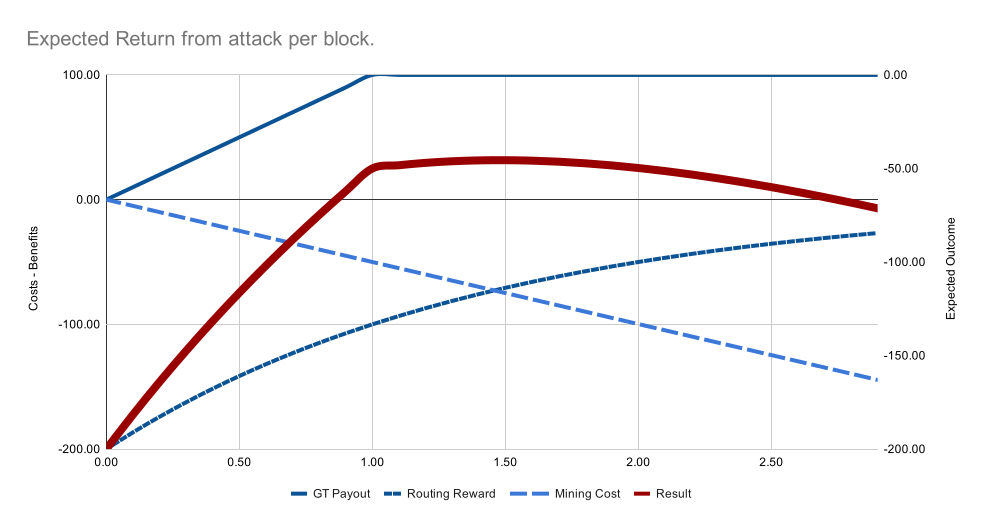
\includegraphics{https://raw.githubusercontent.com/trevelyan/saito-lite/master/docs/svgs/ex1.svg?sanitize=true}
\caption{Example 1}
\end{figure}

Example 3. \textbar{} Parameter \textbar{} Value \textbar{}
\textbar---------------\textbar-------\textbar{} \textbar{} Honest Fees
\textbar{} 100 \textbar{} \textbar{} GT \textbar{} 100 \textbar{}
\textbar{} Attacker Fees \textbar{} 100 \textbar{} \textbar{} Cost/GT
\textbar{} 26 \textbar{} \textbar{} Depth \textbar{} 2 \textbar{}

\begin{figure}
\centering
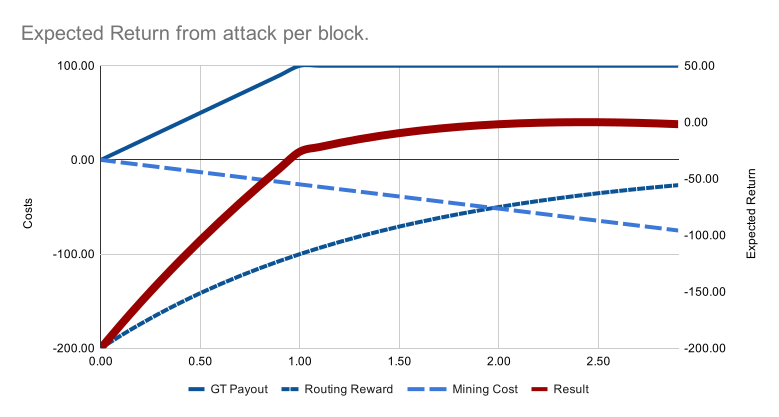
\includegraphics{https://raw.githubusercontent.com/trevelyan/saito-lite/master/docs/svgs/ex3.svg?sanitize=true}
\caption{Example 3}
\end{figure}

\hypertarget{discussion}{%
\subsection{Discussion}\label{discussion}}

In Example 1 we can see that as the miner increases their hashing toward
an average of 1 golden ticket per block, their losses are reduced.
Importantly the reward for the attack is \emph{always} negative.

In Example 2 the attacker is simply mining, not attacking. In this
instance the optimum reward is simply the difference between the reward
for the golden ticket and the cost of producing one. Given difficulty
will push toward mining a golden ticket every second block, an
equilibrium will be reached where mining is porfitable.

In Example 3, we can see that an attack would become profitable if the
golden ticket cost falls below 26. Honest mining would also be
profitable here. Defending the network would simply require mining
profitably such that difficulty pushes the cost per goldent ticket above
this threshold.

In all instances the network remains secure, with attacks on the
mechanism simply defended. At the same time the mechnism can find a
profitable equilibirium for honest operators.

\hypertarget{further-works}{%
\subsection{Further Works}\label{further-works}}

Finiding a generalised proof of the security of the network would be
prove interesting and fruitful work.

\end{document}
